\documentclass[../main.tex]{subfiles}

\begin{document}

\chapter{Geodäten und der Satz von Gauss-Bonnet}

\section{Isometrien}
\section{Paralleltransport und Geodäten}

\begin{goal}
Beschreibe Geodäten $\gamma : \mathbb{R} \to \Sigma$
\end{goal}

\begin{question}
Dazu stellen werden wir folgendes benötigen: Was bedeutet $\dot{\gamma}(t)$ ist konstant?
\begin{itemize}
    \item In $\mathbb{R}^2 \quad \ddot{\gamma}(t)=0$
    \item In $\Sigma \quad \frac{D\dot{\gamma}}{dt}=0$ - die kovariante Ableitung
\end{itemize}
\end{question}

\begin{definition}
Ein glattes Vektorfeld \underline{entlang} einer glatten Kurve $\alpha : [a,b] \to \Sigma$ ist eine glatte Abbildung $w : [a,b] \to \mathbb{R}^3$ mit $w(t) \in T_{\alpha(t)}\Sigma$. \\
Die \underline{horizontale Ableitung} oder ( \underline{kovariante Ableitung} von $w$ im Punkt $\alpha(t)$ ist die orthogonale Projektion der Abbildung $\frac{dw}{dt}(t)$ auf $T_{\alpha(t)}\Sigma :$
\begin{align*}
    \frac{Dw}{dt}(t) = \frac{dw}{dt}(t) - \left\langle \frac{dw}{dt}(t), N(\alpha(t))\right\rangle N(\alpha(t))
\end{align*}
\end{definition}

\begin{remark}
Wir betrachten glatte Kurven und Vektorfelder (aber $C^2$ reicht praktisch immer).
\end{remark}

\subsubsection*{Berechnung in lokalen Koordinaten}
Sei $\varphi : U \to V \subset \Sigma$ eine lokale (glatte) Parametrisierung mit $\alpha([a,b]) \subset \varphi (U) = V$. Schreibe $\varphi^{-1}(\alpha(t))=(u(t),v(t))$.
Sei $w:[a,b]\to \mathbb{R}^3$ ein glattes Vektorfeld entlang $\alpha$. Schreibe $w(t) \in T_{\alpha(t)}\Sigma = \spann \{ \varphi_u, \varphi_v \}$
als $w(t) = \alpha(t)\varphi_u + b(t)\varphi_v$. Es gilt
\begin{align*}
    \frac{dw}{dt}(t) = \dot{a}(t)\varphi_u + \dot{b}\varphi_v + a\dot{u}\varphi_{uu} + a\dot{v}\varphi_{vu} + b\dot{v}\varphi_{vv}
\end{align*}
Dazu erinnere dass $\frac{d}{dt}(\varphi_u = \varphi_{uu}\dot{u} + \varphi_{vu}\dot{v}$
\\
Mit $\varphi_{uu} = eN + \Gamma^1_{11}\varphi_u + \Gamma^2_{11}\varphi_v$ etc.. erhalten wir
\begin{align*}
    \frac{Dw}{dt}(t) = \big(\dot{a} + \Gamma^1_{11}a\dot{u} + \Gamma^1_{12}a\dot{v} + \Gamma^1_{21}b\dot{u} + \Gamma^1_{22}b\dot{v}\big) \varphi_u + \big(\dot{b} + \Gamma^2_{11}a\dot{u} + \Gamma^2_{12}a\dot{v} + \Gamma^2_{21}b\dot{u} + \Gamma^2_{22}b\dot{v}\big) \varphi_v
\end{align*}

\begin{definition}
$w$ heisst \underline{parallel}, falls $\dfrac{Dw}{dt} \equiv 0$ \\ ''keine Änderung in Richtung der Tangentialebene``
\end{definition}

\begin{examples}
\begin{enumerate}
    \item In der Ebene $\mathbb{R}^2 \times \{0\} \subset \mathbb{R}^3$ gilt \begin{align*}
        \frac{Dw}{dt} = \frac{dw}{dt}
    \end{align*}
    Sei $w(t) = a(t)e_1 + b(t)e_2$.
    \begin{align*}
        \frac{dw}{dt} = \dot{a}(t)e_1 + \dot{b}e_2 \perp e_3 = N \implies \frac{Dw}{dt} = \frac{dw}{dt}
    \end{align*}
    
    \item Betrachte $\begin{aligned}[t] \alpha : [0, 2 \pi] & \to S^2 \subset \mathbb{R}^3 \\
    t & \mapsto ( \cos t, \sin t, 0)
    \end{aligned}$ \\
    Dann ist $w(t) \equiv e_3$ ein paralleles Vektorfeld entlang $\alpha$.
    \begin{align*}
        \frac{dw}{dt} = 0 \implies \frac{Dw}{dt} = 0
    \end{align*} beachte hier $e_3 \in T_{\alpha(t)}S^2$ für alle $t$. Weiteres Beispiel $\bar{w}(t) = \dot{\alpha}(t)$ \begin{align*}
        \frac{d \bar{w}}{dt}(t) = \ddot{\alpha}(t) = ( -\cos t, -\sin t, 0) \ || \ N(\alpha(t)) \implies \frac{D\bar{w}}{dt}(t) = 0 \ (\text{ da } \frac{d\bar{w}}{dt} \perp T_{\alpha(t)}S^2 \ )
    \end{align*} 
\end{enumerate}
\end{examples}

\begin{remark}
Die Bedingung $\dfrac{Dw}{dt}=0$ ist unabhängig von der Parametrisierung von $\alpha : [a,b] \to \Sigma $

Sei $\sigma : [a,b] \to [a,b]$ ein Diffeomorphismus mit $\sigma (a) = a$ und $\sigma (b) = b$. Dann gilt
\begin{align*}
    \frac{d}{dt}(w(\alpha(\sigma(t))) = \frac{d}{d\sigma}w(\alpha(\sigma))  \dot{\sigma}(t) \implies \frac{Dw}{dt} = \frac{Dw}{d\sigma}\dot{\sigma}
\end{align*}
\begin{align*}
    \sigma \text{ Diffeomorphismus } & \implies \dot{\sigma}(t) \not = 0 \\
    & \implies \frac{Dw}{dt} = 0 \iff \frac{Dw}{d\sigma} = 0
\end{align*}
\end{remark}

\begin{definition}
Eine glatte Kurve $\gamma : [a,b] \to \Sigma$ heisst \underline{geodätisch}, falls
$\dfrac{D\dot{\gamma}}{dt}\equiv 0 $. Das Bild von $\gamma$ bezeichnen wir mit \underline{Geodäte}.
\end{definition}
Beachte hier $\dot{\gamma}(t) \in T_{\gamma(t)}\Sigma$, also ist $\dot{\gamma}:[a,b] \to \mathbb{R}^3$ ein glattes Vektorfeld entlang $\gamma(t)$.


\begin{examples}
\begin{enumerate}
    \item In der Ebene $\mathbb{R}^2 \times \{0\} \subset \mathbb{R}^3$ gilt $\dfrac{Dw}{dt} = \dfrac{dw}{dt}$ (siehe oben), also 
    \begin{align*}
        \frac{D\dot{\gamma}}{dt}(t)=0 \iff \frac{d\dot{\gamma}}{dt}(t) = \ddot{\gamma}(t) = 0
    \end{align*} Also parametrisieren geodätische Kurven in der Ebene Geradenabschnitte.
    
    \item $\Sigma = S^2, \gamma(t) = (\cos t, \sin t, 0), \gamma : \mathbb{R} \to S^2$ ist geodätisch, da $\frac{D\dot{\gamma}}{dt}(t)=0$. \\
    (Siehe oben: $\frac{d\dot{\gamma}}{dt} = \ddot{\gamma}(t)$ ist parallel zu $N(\gamma(t))$, also senkrecht zu $T_{\gamma(t)}S^2 \implies \frac{D\dot{\gamma}}{dt}=0$.) Analog sind alle \underline{Grosskreisenabschnitte} mit konstanter Geschwindigkeit parametrisiert Geodäten. Wir werden später sehen, dass \underline{alle} Geodäten von dieser Form sind.
    \item $Z = \{(x,y,z) \in \mathbb{R}^3 | x^2 + y^2 = 1\}$
    Betrachte die lokal \underline{isometrische} Parametrisierung.
    $\begin{aligned}[t]
        \varphi : \mathbb{R}^2 & \to Z \\
        (u,v) & \mapsto (\cos u, \sin u, v)
    \end{aligned}$
    \begin{claim}
        Die Bilder von Geodäten in $\mathbb{R}^2$ unter $\varphi$ sind Geodäten.
    \end{claim}
    
    \begin{specialcase}
        Geraden durch $(0,0) \in \mathbb{R}^2$
    \end{specialcase}

\end{enumerate}
\end{examples}
% fehlen noch paar dinge, siehe notizen
\newpage

% Vorlesung 04.05.2022

\begin{recall}
    Eine Kurve $\gamma : \mathbb{R} \to \Sigma$ glatt heisst \emph{geodätisch}, falls
$\dfrac{D\dot{\gamma}(t)}{dt}=0$
\end{recall}

In lokalen Koordinaten bezüglich einer Parametrisierung
$\varphi : U \to \Sigma$, schreibe \\ $\gamma (t) = \varphi(u(t),v(t))$.
(falls $\gamma(\mathbb{R}) \subset \varphi(U)$)

Geodätengleichung
\begin{align*}
    \ddot{u} + \Gamma^1_{11}\dot{u}^2 + 2 \Gamma^1_{12}\dot{u}\dot{v} + \Gamma^1_{22}\dot{v}^2 = 0 \\
    \ddot{v} + \Gamma^2_{11}\dot{u}^2 + 2 \Gamma^2_{12}\dot{u}\dot{v} + \Gamma^2_{22}\dot{v}^2 = 0 
\end{align*}

Führe Koordinaten $w=\dot{u}, z=\dot{v}$ ein. Wir erhalten ein System von Differentialgleichungen 
mit glatten Koeffizienten, (d.h. lokal lipschitz) erster Ordnung auf $\mathbb{R}^4$
\begin{itemize}
    \item $\dot{u} = w$
    \item $\dot{v} = z$
    \item $\dot{w} = \ddot{u} = -(...)$
    \item $\dot{z} = \ddot{v} = -(...)$
\end{itemize}

Es seien Anfangsbedingungen $p \in \Sigma, v \in T_p\Sigma$ vorgegeben $(p\in \varphi(U))$. \\
Seien $(u_0,v_0,w_0,z_0) \in \mathbb{R}^4$ mit $\varphi(u_0,v_0) = p, \  v = w_0\varphi_u+z_0,\varphi_v$
Nach Picard Lindelöf existiert eine \emph{eindeutige} Lösungskurve
$\bar{\gamma}: (-\varepsilon,\varepsilon) \to \mathbb{R}^4$ zur Anfangsbedingung $\bar{\gamma}(0)=(u_0,v_0,w_0,z_0); \ \gamma(t)=(u(t),v(t),w(t),z(t))$.
Dann ist $\gamma(t) = \varphi(u(t),v(t))$ unsere gesuchte Lösung.

$\implies$ \\
\textbf{Proposition 3.} Sei $\Sigma \subset \mathbb{R}^3$ eine glatte reguläre Fläche, $p \in \Sigma$
und $v\in T_p\Sigma$ vorgegeben. Dann existiert $\varepsilon >0$ und eine 
eindeutige geodätische Kurve $\gamma : (-\varepsilon, \varepsilon)\to \Sigma$ mit $\gamma(0)=p$
und $\dot{\gamma}(0)=v$.

\begin{zusatz}
    Für vollständige Flächen (d.h. abgeschlossen und ohne Rand) lässt sich
    $\gamma$ auf $\mathbb{R}$ erweitern.
\end{zusatz}

\begin{remarks}
    \leavevmode
    \begin{enumerate}
        \item Die Geodätengleichungen sind invariant unter Isometrien.\\
        Tätsächlich sind $\Gamma^k_{ij}$ durch die Koeffizientenfunktionen $E,F,G$ bestimmt,
        welche invariant unter Isometrien sind.
        $\implies$ Isometrien bilden Geodäten auf Geodäten ab (auch lokal gültig).

        \item Nach Proposition 3 existiert für alle $p \in \Sigma, v\in T_p\Sigma$ ($\Sigma$ vollständig), genau
        eine geodätische Kurve $\gamma : \mathbb{R} \to \Sigma$ mit $\gamma(0)=p, \dot{\gamma}(0)=v$.
        Falls wir für alle Paare $(p,v)$ schon eine Geodäte kennen, dann haben wir alle
        Geodäten gefunden. \\
        \emph{Anwendung}: Geodäten auf $S^2$ sind \emph{Grosskreise}. \\
        Geodäten auf dem Zylinder $Z$ sind \emph{Helixen, Meridiane, Mantellinien}.
    \end{enumerate}
\end{remarks}

\section{Exponentialabbildung und geodätische Polarkoordinaten}

Sei $\Sigma \subset \mathbb{R}^3$ glatt und vollständig, sowie $p\in \Sigma, \ v\in T_p\Sigma,
\gamma : \mathbb{R} \to \Sigma$ die eindeutige geodätische Kurve mit 
$\gamma (0)=p, \dot{\gamma}(0) =v$
\begin{notation} $\gamma_p (v,t) = \gamma(t)$
\end{notation}

\begin{definition}
    $\begin{aligned}[t]
        \exp : T_p\Sigma & \to \Sigma \\
        v & \mapsto \gamma_p(v,1) 
    \end{aligned}$ \qquad
    \tikzfig{exponentialabbildung}
\end{definition}


\begin{remarks}

\leavevmode
\begin{enumerate}
    \item Es gilt für alle $\lambda > 0, t \in \mathbb{R}$: $\gamma_p(\lambda v, t) = \gamma_p(v,\lambda t)$
    \item Eine Verschärfung des Satzes von Picard-Lindelöf nach Cauchy zeigt,
    dass die Lösung $\gamma_p(v,t)$ glatt von den Parametern $p \in \Sigma, v \in T_p\Sigma$, und
    $t\in \mathbb{R}$ abhängt. Daraus folgt, dass $\exp : T_p\Sigma \to \Sigma$ glatt ist!

    \item Wieso heisst diese Abbildung $\exp$?
    Die Antwort kommt aus der Lietheorie: 
    Betrachte die Gruppe $GL(\mathbb{C}^n)$. Für $A \in \mathbb{C}^{n \times n}$ haben
    wir die Abbildung $\gamma(t)= e^{tA} \in GL(\mathbb{C}^n)$.
    Diese Kurve ist geodätisch bezüglich der Killingform auf $GL(\mathbb{C}^n)$\\
    $\ulcorner$ Sei $X \in GL(\mathbb{C}^n)$ und $A,B \in T_XG(\mathbb{C}^n)$

    $\langle A, B \rangle = spur (X^{-1}AX^{-1}B)?$ Stimmt für $X = Id$
    $\lrcorner$ 
\end{enumerate}

\end{remarks}

\subsubsection*{Berechung des Differentials von exp} 
Sei $p \in \Sigma$ und $h \in T_p\Sigma$ und $\gamma : \mathbb{R} \to \Sigma$
die eindeutige geodätische Kurve mit $\gamma(0)=p$ und $ \dot{\gamma}(0)=h$, also
$\exp (th)= \gamma_p(th,1) = \gamma_p(h,t)=\gamma(t)$.
Berechne nun:
\begin{align*}
    (D\exp)_0(h) = \lim_{t \to 0}\frac{\exp(th)-\exp(0)}{t} =
    \lim_{t \to 0} \frac{\gamma(t)-\gamma(0)}{t} =\dot{\gamma}(t)=h \\
    \implies D(\exp)_0 = \text{Id}_{T_p\Sigma}  
\end{align*}

Nach Umkehrsatz existiert eine Zahl $\delta > 0$, so dass die Einschränkung
von $\exp$ auf $U=T_p\Sigma \cap B_0(\delta) = \{v \in T_p\Sigma \ | \ ||v||_2 < \delta \}$
ein Diffeomorphismus ist. Insbesondere ist 
$\varphi = \exp \vert_U : U \to \varphi(U) \subset \Sigma$ eine lokale Parametrisierung. \\
\begin{minipage}{30em}
    Wähle auf $T_p\Sigma$ Polarkoordinaten $(r, \theta)$ (Wahl ist wo ist $\theta = 0$?).
Die entsprechenden Koordinaten auf $\exp (U) \subset \Sigma$ heissen \emph{geodätische
Polarkoordinaten}.
\end{minipage}
\begin{minipage}{10em}
    \ctikzfig{differential}
\end{minipage}



\begin{proposition}
    Bezüglich der lokalen Parametrisierung $\varphi = \exp : U \to \Sigma$
    und Koordinaten $(u,v) = (r, \theta)$ gilt: $$E=1, F=0,\lim_{r \to 0} G(r,\theta)=0
    \text{ und } \lim_{r \to 0} \frac{d}{dr}\sqrt{G(r,\theta)} = 1$$

\end{proposition}

\begin{proof}
    Fixiere einen Winkel $\theta \in S^1 = [0,2\pi] / 0 = 2\pi$.
    Es gilt $E(r,\theta) = \left \langle \dfrac{d}{dr} \exp, \dfrac{d}{dr}\exp \right\rangle$.
    Da die Kurve $ t \to \exp (t, \theta)$ geodätisch mit Geschwindigkeit $1$ ist,
    folgt $$\left|\left| \frac{d}{dr}\exp (r, \theta)\right|\right| = 1 \implies E(r,\theta)=1$$
    Das Paar $(r, \theta)$ erfüllt die Geodätengleichung:
    $$
        \ddot{\theta} + \Gamma^2_{11}\dot{r}^2 + 2 \Gamma^2_{12}\dot{r}\dot{\theta} + \Gamma^2_{22}\dot{\theta}^2 = 0 
    $$
    Da $\theta$ konstant ist, folgt $\Gamma^2_{11}=0$. Weiterhin gilt (siehe Abschnitt Theorema Egregium)

    $$
    \begin{pmatrix}
        E & F \\ F & G
    \end{pmatrix}
    \begin{pmatrix}
        \Gamma^1_{11} \\ \Gamma^2_{11} % das zweite = 0
    \end{pmatrix} = 
    \begin{pmatrix}
        \frac{1}{2}E_r \\ F_r - \frac{1}{2}E_{\theta}
    \end{pmatrix} \qquad \text{wobei }\Gamma^2_{11}=0
    $$$ E = 1 \implies E_r = E_{\theta} = 0 \implies \Gamma^1_{11}=0 \text{ und } F_r =0$.
    Also hängt $F(r,\theta) = \langle \exp _r, \exp _{\theta} \rangle$
    nicht von von $r$ ab!

    Mit $\lim_{r \to 0} ||\exp _{\theta} || = 0 $ folgt also $F = 0$.    
    Ausserdem folgt mit $\lim_{r \to 0} ||\exp _{\theta}|| = 0$ auch 
    $\lim_{r \to 0} G(r,\theta) = \lim_{r \to 0} \langle \exp _{\theta}, \exp _{\theta} \rangle = 0$.

    Genauer: In erster Ordnung in $r$ gilt $||\exp_{\theta}(r,\theta)|| = r$ (+höhere Terme)
    also $$\lim_{r \to 0} \frac{d}{dr}\sqrt{G(r,\theta)} = \lim_{r \to 0} \frac{d}{dr} ||\exp_{\theta}(r,\theta)|| =1
    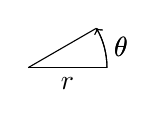
\begin{tikzpicture}
        \draw (0,0) -- (1,0)
            node[midway, below] {$r$};
        \draw (0,0) -- (0.866,0.5);
        \draw[->] (1,0) arc (0:30:1 and 1)
            node[midway, right] {$\theta$};
            \draw[->] (1,0) arc (0:30:1 and 1)
            node[midway, right] {$\theta$};
    \end{tikzpicture}$$
\end{proof}

\subsubsection*{Krümmung in geodätischen Polarkoordinaten}
Wir betrachten eine lokale Parametrisierung $\exp : U \to \Sigma$. Bezüglich Polarkoordinaten $(r, \theta)$ auf $U \subset \mathbb{R}^2$ gilt: \\
$E=1, F=0, \Gamma^1_{11}=\Gamma^2_{11}=0$.

Weiterhin gilt:
$$
\underbrace{\begin{pmatrix}
    E & F \\ F & G
\end{pmatrix}}_{= \begin{pmatrix}
    1 & 0 \\ 0 & G
\end{pmatrix}}
\begin{pmatrix}
    \Gamma^1_{12} \\ \Gamma^2_{12}
\end{pmatrix} = 
\begin{pmatrix}
    \frac{1}{2}E_{\theta} \\ \frac{1}{2}G_r
\end{pmatrix} =
\begin{pmatrix}
    0 \\ \frac{1}{2}G_r
\end{pmatrix} \implies G\Gamma^2_{12} = \frac{1}{2}G_r
$$

Berechnung der Krümmung mittels der Formel (Lemma, Theorema Egregium).
\begin{align*}
    -EK = -K & = (\Gamma^2_{12})_r + (\Gamma^2_{12})^2 \qquad \text{Viele Terme streichen sich weg}\\
    & = \frac{d}{dr}\left(\frac{1}{2}\frac{G_r}{G}\right) + \left(\frac{1}{2}\frac{G_r}{G}\right)^2 \text{benutze $G\not =0,$ da $\det \not = 0$}
\end{align*}

\begin{proposition}
    $K = -\dfrac{(\sqrt{G})_{rr}}{\sqrt{G}}$
\end{proposition}
\begin{proof}
    \begin{align*}
        K = -\frac{(\sqrt{G})_{rr}}{\sqrt{G}} & = - \frac{1}{\sqrt{G}}\left(\frac{1}{2}\frac{G_r}{\sqrt{G}}\right)_r \\
        & = -\frac{1}{2}\frac{G_{rr}}{G} + \frac{1}{4}\frac{(G_r)^2}{G^2} \\
        & = -\frac{1}{2}\left(\frac{G_r}{G}\right)_r - \frac{1}{4}\frac{G_r^2}{G^2} = K
    \end{align*}
\end{proof}

\begin{application}
Sei $\Sigma \subset \mathbb{R}^3$ eine glatte reguläre Fläche, und $\exp : U \to \Sigma$ eine lokale Parametrisierung.
Wir machen für die Koeffizientenfunktion $\sqrt{G(r,\theta)}$ eine Taylorentwicklung.
\begin{ansatz}
Unter Berücksichtigung von $\lim_{r \to 0}\sqrt{G}=0, \lim_{r \to 0}\sqrt{G}_r=1$, sowie Prop. 4
$\sqrt{G}=r + a (\theta)r^2 + b(\theta)r^3 + ...$, (Restterm $R(r,\theta)$ erfüllt $\lim_{r \to 0}\frac{1}{r^3}R(r,\theta)=0)$

$$\implies \sqrt{G}_{rr}= 2a(\theta) + 6b(\theta)r + \text{höhere Terme}$$
Prop. 5$$ \implies K = - \frac{\sqrt{G}_{rr}}{\sqrt{G}}=\frac{2a(\theta)+6b(\theta)r+ ...}{r + a(\theta)r^2 + b(\theta)r^3 + ...}$$
Die Grenzbetrachtung $r \to 0$ liefert:
\begin{itemize}
    \item $a(\theta)=0$ (da K nicht $\to \infty$ gehen darf wegen Glattheit)
    \item $b(\theta) =\dfrac{K}{6}$.
\end{itemize}
Damit erhalten wir $\sqrt{G}=r- \frac{K}{6}r^3 + R(r,\theta)$
Sei $p\in \Sigma$ und $r >0$.
\begin{definition}
    Definiere $K^{\Sigma}(p,r)=\exp(K_0(r))$, wobei $K_0(r)=\{z\in T_p\Sigma | \ |z|=r\}$\\
    ''Kreis um p in $\Sigma$ mit Radius $r$, \emph{den Kreis runterlegen}``
\end{definition}

\end{ansatz}

Setze $U^{\Sigma}(p,r)=$Länge$(K^{\Sigma}(p,r))= \int_{0}^{2\pi}\sqrt{G}  \,d\theta $. Weglänge war definiert $\int_{0}^{t} \sqrt{E \dot{u}^2+ 2F \dot{u}\dot{v}+G\dot{v}^2 }\,dt $ hier $u =r, v = \theta$.

\end{application}
\begin{theorem}[Umfangdefektformel]
    $$K(p)=\lim_{r \to \theta} \frac{2\pi r - U^{\Sigma}(p,r)}{r^3}\frac{3}{\pi}$$
\end{theorem}
\begin{proof}
    Berechne
    \begin{align*}
        U^{\Sigma}(p,r) &= \int_{0}^{2\pi} \sqrt{G(r,\theta)} \,d\theta  \\ 
        &= \int_{0}^{2\pi}[r- \frac{K(p)}{6}r^3 + R(r,\theta)] \,d\theta \\
        &= 2\pi r -\frac{2\pi}{6}K(p)r^3 + \int_{0}^{2\pi} R(r,\theta) \,d\theta  \\
        & \implies \lim_{r \to 0} \frac{2\pi r - U^{\Sigma}(p,r)}{r^3} = \frac{\pi}{3}K(p)
    \end{align*}
\end{proof}
\begin{geometric}

\ctikzfig{curvatures}

\end{geometric}
\begin{application}[Flächen konstanter Krümmung]
Falls $K$ konstant ist, dann hat die Differentialgleichung 
$ K \sqrt{G}= - \sqrt{G}_{rr}$ zur Anfangsbedingung $\sqrt{G}(0,\theta)=0$
$\sqrt{G}_r(0,\theta)=1$ siehe Prop. 4 eine eindeutige Lösung:
\leavevmode
\begin{enumerate}
    \item $K=0 \implies \sqrt{G(r,\theta)}=r$ also $G=r^2$
    \item $K > 0 \implies \sqrt{G(r,\theta)}= \dfrac{1}{\sqrt{K}}\sin (\sqrt{K}r)$ also $G=\dfrac{1}{K}\sin (\sqrt{K}r)^2$
    \item $K < 0 \sqrt{G(r, \theta)}=\dfrac{1}{\sqrt{-K}} \sinh (\sqrt{-K}r)$ wobei $\sinh (x)=\frac{1}{2}(e^x - e^{-x})$
\end{enumerate}  
In allen Fällen ist $G$ unabhängig von $\theta$!
\end{application}

Kreisumfang:
\begin{itemize}
    \item $K=0$ siehe Weglänge $\int_0^T \sqrt{\dot{r}^{2}E + \dot{u}\dot{v}F + \dot{v}^2 G} \ dt $\\
    $$U(r)= \int_0^{2\pi} \sqrt{G} \ d\theta = \int_0 ^{2\pi} r \ d\theta = 2\pi r$$
    \item $K=1$ mit $\sin(x)=x-\frac{x^3}{3!} + \dots$ \\
    $$U(r) = \int_0^{2\pi} \sqrt{G} \ d\theta = 2 \pi \sin(r)$$
    \item $K=-1$ ``Umfang wächst exponentiell''\\
    $$U(r)=2\pi \sinh (r) \sim e^r$$
\end{itemize}

\begin{theorem}[Minding 1839]
    Seien $\Sigma_1, \Sigma_2$ reguläre Flächen mit derselben konstanten Krümmung $K$, und $p_1 \in \Sigma_1,p_2 \in \Sigma_2$.
    Dann existiert $U_1 \subset \Sigma_1, U_2 \subset \Sigma_2$ offen mit $p_i \in U_i$ und eine lokale Isometrie $h : U_1 \to U_2$.
\end{theorem}

\begin{proof}
    Bezüglich geodätischer Polarkoordinaten um $p_1, p_2$ sind die Koeffizientenfunktionen $E=1, F=0, G$ durch $K$ bestimmt, also identisch.
    Wir folgern, dass $\Sigma_1, \Sigma_2$ lokal isometrisch sind (siehe Abschnitt Isometrien).
\end{proof}

\section{Der Satz von Gauss-Bonnet}
\begin{minipage}{30em}
    Sei $\Sigma \subset \mathbb{R}^3$ eine glatte reguläre Fläche. Wir betrachten das Standarddreieck $\triangle \subset \mathbb{R}^3$ mit Eckpunkten $e_1,e_2,e_3$.
\end{minipage}
\begin{minipage}{8em}
    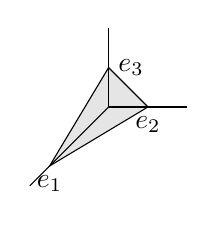
\begin{tikzpicture}
        \filldraw[fill = gray!20] (-0.75,-0.75) node[below] {$e_1$} -- (0,0.5) node[right] {$e_3$}-- (0.5,0) node[below] {$e_2$}-- cycle;
        \draw (0,0) -- (-1,-1);
        \draw (0,0) -- (1,0);
        \draw (0,0) -- (0,1);
    \end{tikzpicture}
\end{minipage}

Ein Dreieck in $\Sigma$ ist das Bild von $\triangle$ unter einer glatten Abbildung $\varphi : \triangle \to \Sigma$.
Falls die Kanten von $\varphi (\triangle)$ Segmente von Geodäten sind, dann heisst das Dreieck geodätisch.

\begin{definition}
    Ein \emph{geodätisches Dreieck} in $\Sigma \subset \mathbb{R}^3$ ist ein eingebettetes Dreieck, welches von drei geodätischen Segmenten begrenzt wird.
\end{definition}

\begin{theorem}[Lokale Version von Gauss-Bonnet]
    Sei $\triangle \subset \Sigma$ ein geodätisches Dreieck mit Innenwinkeln $\alpha, \beta, \gamma$. Dann gilt
    \begin{align*}
        \int_{\triangle} K \,dA = \alpha + \beta + \gamma - \pi 
    \end{align*}
\end{theorem}
 
\begin{recall}
    \emph{Flächenelement} $dA = \sqrt{EG-F^{2}}$ 
\end{recall}

\begin{remark}
    Bei konstanter Krümmung $K = 0$ haben alle geodätischen Dreiecke die Innenwinkelsumme $\pi$
\end{remark}

\begin{geometric}
    \ctikzfig{geodesicTriangleTheorem}
\end{geometric}

\begin{preparation}
Additivität der Formel:
$\triangle = \triangle _1 \cup \triangle _2$

\begin{minipage}{8em}
    \tikzfig{triangleAdditivity}
\end{minipage}
\begin{minipage}{32em}
    $$\underbrace{\int_{\triangle} K \ dA}_{\alpha + \beta + \gamma - \pi } = \underbrace{\int_{\triangle_1}K \ dA }_{\alpha_1 + \beta_1 + \gamma_1 - \pi}+ \underbrace{\int_{\triangle_2}K \ dA}_{\alpha_2 + \beta_2 + \gamma_2 - \pi}$$
    Ok, da $\alpha + \beta + \gamma - \pi = \alpha_1 + \beta_1 + \gamma_1 - \pi + \alpha_2 + \beta_2 + \gamma_2 - \pi$
\end{minipage}
\begin{minipage}{8em}
    \tikzfig{triangleAdditivityVariant}
\end{minipage}
\begin{minipage}{32em}
    $$\sum_{i=1}^{3} \alpha_i + \beta_i + \gamma_i = \alpha + \beta + \gamma + 2\pi \implies \int_{\triangle}K \ dA = \sum_{i=1}^{3}\int_{\triangle_i}K \ dA$$
\end{minipage}
\end{preparation}

\begin{proof}
    Wir nehmen zunächst an, es gäbe eine lokale Parametrisierung der Form
    \(\varphi = exp : U \to \Sigma\) mit \(\triangle_A \subset \varphi(U)\)
    und \(\varphi(0)\) sei ein Eckpunkt von $\triangle$, ebenso sei $B \in \varphi (U\cap \mathbb{R} \times \{0\})$
    
    \begin{figure}[htb]
        \centering
        \def\svgwidth{40em}
        \input{figures/triangleExp.pdf_tex}
        \caption{Interpretation von exp}        
    \end{figure}


Parametrisiere den Weg $\delta : [0,\alpha] \to \Sigma$ durch $\delta(\theta) = \exp(r(\theta), \theta)$. Berechne
\begin{align*}
    \int_{\triangle} K \,dA & = \int_{\varphi^{-1}(\triangle)} K(r,\theta) \sqrt{EG-F^{2}}\,drd\theta \\
    & \overset{E=1, F=0, \text{ da } \varphi = \exp}{=}\int_{\varphi^{-1}(\triangle)} K\sqrt{G}  \,drd\theta \\ 
    & \overset{\text{Prop. 5}}{=} \int_{\varphi^{-1}(\triangle)} -\sqrt{G}_{rr} \ drd\theta \\
    & = - \int_{0}^{\alpha} \int_{0}^{r(\theta)} \sqrt{G}_{rr}\,drd\theta \\
    & = - \int_{0}^{\alpha} \left [\sqrt{G}_r (r(\theta), \theta) - \sqrt{G}_r(0,\theta) \right ] \,d\theta \\
    & = \alpha - \int_{0}^{\alpha} \sqrt{G}_r (r(\theta,\theta))  \,d\theta 
\end{align*}

\begin{lemma*}
    \begin{align*}
        -\sqrt{G}_r (r(\theta, d\theta)) = \frac{\partial \psi}{\partial \theta}
    \end{align*} wobei $\psi(\theta)$ der Winkel zwischen $e_r$ und $\dot{\delta}(\theta)$ ist.
\end{lemma*}

\begin{figure}[htb]
    \centering
    \def\svgwidth{20em}
    \input{figures/interpretation.pdf_tex}
    \caption{Darstellung von Lemma}        
\end{figure}

Insbesondere gilt $\psi (0) = \pi - \beta $ und $\psi (\alpha) = \gamma$. Mit dem Lemma folgt also
\begin{align*}
    \int_{\triangle} K  \,dA &= \alpha + \int_{0}^{\alpha} \frac{\partial \psi}{\partial \theta} \,d\theta \\
    &= \alpha + \psi(\alpha) - \psi(0) \\
    &= \alpha + \beta + \gamma - \pi
\end{align*}
\end{proof}

\begin{proof}[Lemma]
    Berechne 
    \begin{align*}
        \sqrt{G}_r = \frac{1}{2} \frac{G_r}{\sqrt{G}} = \frac{1}{2\sqrt{G}} \frac{\partial}{\partial r} \underbrace{\langle \varphi_{\theta} , \varphi_{\theta} \rangle}_{=G} \\
        = \frac{1}{\sqrt{G}} \langle \varphi_{r\theta}, \varphi_{\varphi_\theta} \rangle = \langle \frac{\partial \varphi _r}{\partial \theta} , \frac{\varphi_{\theta}}{||\varphi _{\theta}||} \rangle
    \end{align*} wobei im letzten Schritt $\varphi_{r\theta} = \varphi_{\theta r}$ und $\sqrt{G} = ||\varphi_{\theta}||$ verwendet wird.
    Wir erinnern uns daran, dass
    $$\left \langle \frac{\partial \varphi_r}{\partial \theta}, \frac{\varphi _{\theta}}{||\varphi_{\theta}||} \right \rangle = -\frac{\partial \psi}{\partial \theta}$$
    ``Die Winkeländerung von $\psi$ und $\varphi_r$ stimmen überein.''
\end{proof}

\begin{figure}[htb]
    \centering
    \def\svgwidth{30em}
    \input{figures/proof_geometric.pdf_tex}
    \caption{Beweis geometrisch}        
\end{figure}

\begin{remark}
    Falls $\triangle \subset \Sigma$ nicht im Bild einer Parametrisierung
    $\varphi = \exp : U \to \Sigma $ liegt, unterteile $\triangle$ iteriert, bis alle Teildreiecke diese Eigenschaft haben.
\end{remark}

\begin{figure}[htb]
    \centering
    \def\svgwidth{10em}
    \input{figures/triangle.pdf_tex}
    \caption{Iterationsschritt (Seiten halbieren)}        
\end{figure}

\end{document}
